\addcontentsline{toc}{chapter}{Занятие 4. Гауссовские процессы}
\chapter*{Занятие 4. Гауссовские процессы}

\addcontentsline{toc}{section}{Контрольные вопросы и задания}
\section*{Контрольные вопросы и задания}

\subsubsection*{Приведите определение гауссовского процесса.}

Процесс $ \left\{ X \left( t \right), \, t \in T \right\} $ --- гауссовский, если
$$ \sum \limits_{k = 1}^n \lambda_k X \left( t_k \right) $$
--- гауссовская случайная величина $ \forall \vec{ \lambda } \in \mathbb{R}^n$ и
$ \forall t_1, \dotsc, t_n \in T$.

Эквивалентно: $ \left( X \left( t_1 \right), \dotsc, X \left( t_n \right) \right)^T$ ---
гауссовский вектор.

\subsubsection*{Запишите плотность конечномерных распределений гауссовского процесса.}

$$p =
  \frac{1}{ \left( \sqrt{2 \pi} \right)^n} \cdot \frac{1}{ \sqrt{det \, A}} \cdot
  e^{-\frac{1}{2} \left[ A^{-1} \left( \vec{x} - \vec{a} \right), \vec{x} - \vec{a} \right] },$$
если $det \, A > 0$.
Квадратные скобки в степени экспоненты --- это скалярное произведение,
или квадратичная форма матрицы, обратной к ковариации.

\subsubsection*{Приведите определение и сформулируйте основные свойства ковариационной функции.}

$K \left( t, s \right) =
  cov \left[ X \left( t \right), X \left( s \right) \right] $.

Гауссовский процесс существует, из теомеры Колмогорова, с функциями $m$ и $K$ тогда и только тогда,
когда функция $K \left( s, t \right) = K \left( t, s \right) $ --- симметричная, и $K$ ---
неотрицательно определённая, то есть
$$ \sum \limits_{k, j = 1}^n c_k c_j K \left( t_k, t_j \right) \geq
  0.$$

Тут неравенство возможно для любых $c_1, \dotsc, c_n, t_1, \dotsc, t_n$.

\subsubsection*{4.2}

\textit{Задание.}
Выясните, существует ли случайный процесс с ковариационной функцией
\begin{enumerate}[label=\alph*)]
  \item $K \left( t, s \right) = \min \left( t, s \right) $;
  \item $K \left( t, s \right) =
    \left( 1 - \left| t - s \right| \right) \cdot
    \mathbbm{1} \left\{ \left| t - s \right| < 1 \right\}; \,
    t, s \in \mathbb{R}$.
\end{enumerate}

\textit{Решение.}
\begin{enumerate}[label=\alph*)]
  \item $K \left( t, s \right) = \min \left( t, s \right) $.

  Такой процесс есть.
  Какой?
  Винеровский;
  \item $K \left( t, s \right) =
    \left( 1 - \left| t - s \right| \right) \cdot
    \mathbbm{1} \left\{ \left| t - s \right| < 1 \right\}; \,
    t, s \in \mathbb{R}$.

  Если такой процесс есть, то мы его не встречали раньше.
  Симметричность очевидна.
  Вопрос: будет ли такая функция неотрицательно определена?

  Функция зависит только от разности.
  Сейчас $K \left( t, s \right) = \varphi \left( t - s \right) $, где
  $$ \varphi \left( t, s \right) =
    \begin{cases}
      1 - \left| t \right| , \qquad \left| t \right| \leq 1, \\
      0, \qquad \left| t \right| > 1.
    \end{cases}$$
  Так что
  $$ \sum \limits_{k, j = 1}^n c_k c_j K \left( t_k, t_j \right) =
    \sum \limits_{k, j = 1}^n c_k c_j \varphi \left( t_k - t_j \right) \geq
    0$$
  --- это условие неотрицательной определённости для характеристической функции.
  Будет ли эта функция $ \varphi $ характеристической?
  То есть вопрос в задаче равносилен следующему: будет ли
  $$ \varphi \left( t \right) =
    \begin{cases}
      1 - \left| t \right| , \qquad \left| t \right| \leq 1, \\
      0, \qquad \left| t \right| > 1.
    \end{cases}$$
  характеристической функцией?
  Эта функция изображена на рисунке \ref{fig:42}.

  \begin{figure}[h!]
    \centering
    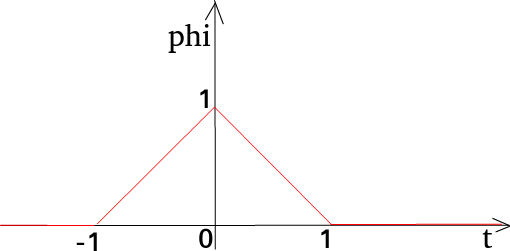
\includegraphics[width=.4\textwidth]{./pictures/4_2.png}
    \caption{График функции $ \varphi \left( t \right) $}
    \label{fig:42}
  \end{figure}


  Она непрерывная, симметричная, в нуле --- единица.
  Если бы это была характеристическая функция
  $$ \varphi \left( t \right) =
    \int \limits_{-\infty }^{+\infty } e^{itx} p \left( x \right) dx$$
  --- преобразование Фурье плотности $p \left( x \right) $.
  Плотность можно найти через обратное преобразование Фурье
  $$p \left( x \right) =
    \frac{1}{2 \pi } \int \limits_{-\infty}^{+\infty } e^{-itx} \varphi \left( t \right) dt =
    \frac{1}{2 \pi } \int \limits_{-1}^1 e^{-itx} \left( 1 - \left| t \right| \right) dt =$$
  Раскроем модуль
  $$= \frac{1}{2 \pi } \left(
    \int \limits_{-1}^1 e^{-itx} dt + \int \limits_{-1}^0 e^{-itx} tdt -
    \int \limits_0^1 e^{-itx} tdt \right) =$$
  Берём первый интеграл
  $$= \frac{1}{2 \pi } \left(
    \left. -\frac{e^{-itx}}{ix} \right|_{-1}^1 - \int \limits_0^1 e^{itx} tdt -
    \int \limits_0^1 e^{-itx} tdt \right) =$$
  Подставляем пределы интегрирования
  $$= \frac{1}{2 \pi } \left[
    -\frac{e^{-ix}}{ix} + \frac{e^{ix}}{ix} -
    \int \limits_0^1 \left( e^{-itx} + e^{itx} \right) tdt \right] =$$
  Из формулы Эйлера следует, что $e^{-itx} + e^{itx} = 2 \cos \left( tx \right) $.
  Тогда
  $$= \frac{1}{2 \pi }
    \left[ \frac{-e^{-ix} + e^{ix}}{ix} - 2 \int \limits_0^1 \cos \left( tx \right) tdt \right] =$$
  Интегрируем по частям, то есть
  $$u = t, \,
    du = dt, \,
    dv = \cos \left( tx \right) dt, \,
    c = \int \cos \left( tx \right) dt = \frac{1}{x} \cdot \sin \left( xt \right).$$
  Получаем
  $$= \frac{1}{2 \pi } \left[
      \frac{-e^{-ix} + e^{ix}}{ix} -
      2 \cdot \left. \frac{t}{x} \cdot \sin \left( xt \right) \right|_0^1 +
      2 \int \limits_0^1 \frac{1}{x} \cdot \sin \left( xt \right) dt \right] =$$
  Подставляем пределы интегрирования и берём интеграл от синуса
  $$= \frac{1}{2 \pi } \left[
    \frac{-e^{-ix} + e^{ix}}{ix} - \frac{2}{x} \cdot \sin x -
    \left. \frac{2}{x^2} \cdot \cos \left( xt \right) \right|_0^1 \right] =$$
  Снова подставляем пределы интегрирования
  $$= \frac{1}{2 \pi } \left(
    \frac{-e^{-ix} + e^{ix}}{ix} - \frac{2}{x} \cdot \sin x - \frac{2}{x^2} \cdot \cos x +
    \frac{2}{x^2} \right) =$$
  Из формулы Эйлера следует, что $e^{ix} - e^{-ix} = 2i \sin x$.
  Тогда
  $$= \frac{1}{2 \pi} \left[
    \frac{2 \sin x}{x} - \frac{2 \sin x}{x} + \frac{2}{x^2} \left( -\cos x + 1 \right) \right] =
  \frac{1}{ \pi x^2} \left( 1 - \cos x \right).$$

  Нашли обратное преобразование Фурье
  $$ \varphi \left( t \right) =
    \int \limits_{-\infty }^{+\infty } e^{itx} p \left( x \right) dx $$
  и $p \left( x \right) \geq 0$.

  Должно выполняться условие нормировки
  $$ \int \limits_{-\infty }^{+\infty } p \left( x \right) dx =
    \varphi \left( 0 \right) =
    1.$$
  Так что $p$ --- плотность, $ \varphi $ --- это её преобразование Фурье, так что $ \varphi $ ---
  характеристическая функция.
  \end{enumerate}

\subsubsection*{4.3}

\textit{Задание.}
Пусть $K \left( t, s \right), \, t, s \in T$ ---
ковариационная функция некоторого случайного процесса, $Q \left( t \right) $ ---
полином с положительными коэффициентами.
Докажите, что функция $K_1 \left( t, s \right) = Q \left( K \left( t, s \right) \right) $
тоже является ковариационной функцией некоторого случайного процесса.

\textit{Решение.}
$Q \left( t \right) = a_0 + a_1 t + a_2 t^2 + \dotsc + a_n t^n, \, a_0, a_1, \dotsc, a_n \geq 0$.
Доказать, что если в этот многочлен подставить ковариационную функцию,
то снова получится ковариационная функция.

Явно запишем, что такое
$$K_1 \left( t, s \right) =
  a_0 + a_1 K \left( t, s \right) + a_2 K \left( t, s \right)^2 + \dotsc +
  a_n K \left( t, s \right)^n.$$

Симметричность есть, так как $K \left( t, s \right) $ --- симметрична.

Задачу можно разбить на две подзадачи:
\begin{enumerate}
  \item если $R_0, R_1, R_2, \dotsc, R_n$ --- ковариационные функции, то и
  $$ \sum \limits_{j = 0}^n a_j R_j \left( t, s \right) $$
  --- ковариационная функция.
  Это утверждение проверить просто.

  Доказательство.
  Берём двойную сумму
  $$ \sum \limits_{k, i = 1}^n
    c_k c_i \left( \sum \limits_{j = 0}^n a_j R_j \left( t_k, t_i \right) \right) =$$
  Меняем суммы местами
  $$= \sum \limits_{j = 0}^n
    a_j \left( \sum \limits_{k, i = 1}^n R_j \left( t_k, t_i \right) c_k c_i \right) \geq 0,$$
  так как внутренняя сумма неотрицательна.
  Так что 1. проверили;
  \item чтобы 1. применить, достаточно проверить, что степень ковариационной функции ---
  это тоже ковариационная функция.
  Достаточно проверить, что если $R_1, R_2$ --- ковариационные функции,
  то и произведение $R_1 \left( t, s \right) R_2 \left( t, s \right) $ ---
  тоже ковариационная функция.

  Условие неотрицательности сейчас записывается так
  $$ \sum \limits_{k, j = 1}^n c_k c_j R_1 \left( t_k, t_j \right) R_2 \left( t_k, t_j \right) \geq
    0?,$$
  где
  $R_1 \left( t_k, t_j \right) = M \left[ X \left( t_k \right) X \left( t_j \right) \right], \,
    R_2 \left( t_k, t_j \right) = M \left[ Y \left( t_k \right) Y \left( t_j \right) \right] $.

  Раз $R_1$ --- ковариационая и $R_2$ --- ковариационная,
  то существуют независимые процессы $X \left( t \right) $ и $Y \left( t \right) $, такие, что
  $$R_1 \left( t, s \right) = M \left[ X \left( t \right) X \left( s \right) \right], \,
    R_2 \left( t, s \right) = M \left[ Y \left( t \right) Y \left( s \right) \right].$$
  Тогда если возьмём новый процесс
  $$Z \left( t \right) = X \left( t \right) Y \left( t \right),$$
  то
  $M \left[ Z \left( t \right) Z \left( s \right) \right] =
    M \left[ X \left( t \right) Y \left( t \right) X \left( s \right) Y \left( s \right) \right] $.
  Группируем первый множитель с третьим, второй --- с четвёртым, пользуемся независимостью
  $M \left[ X \left( t \right) Y \left( t \right) X \left( s \right) Y \left( s \right) \right] =
    M \left[ X \left( t \right) X \left( s \right) \right] \cdot
    M \left[ Y \left( t \right) Y \left( s \right) \right].$
  По введённым обозначениям
  $M \left[ X \left( t \right) X \left( s \right) \right] \cdot
    M \left[ Y \left( t \right) Y \left( s \right) \right] =
    R_1 \left( t, s \right) R_2 \left( t, s \right) $.
\end{enumerate}

\subsubsection*{4.4}

\textit{Задание.}
Пусть $ \left\{ S_n, \, n = 0, 1, 2, \dotsc \right\} $ являетс простым случайным блужданием,
что определяется следующим образом $S_0 = 0; \, S_{n + 1} = S_n + \varepsilon_{n + 1}$,
где $ \left\{ \varepsilon_n \right\}_{n \geq 1}$ ---
последовательность независимых одинаково распределённых случайных величин таких, что
$$P \left( \varepsilon_i = 1 \right) =
  P \left( \varepsilon_i = -1 \right) =
  \frac{1}{2}.$$
Вычислите математическое ожидание и ковариационную функцию процесса
$ \left\{ S_n, \, n = 0, 1, 2, \dotsc \right\} $.
Докажите, что
$$ \frac{S_n}{ \sqrt{n}} \overset{d}{ \to } N \left( 0, 1 \right), \,
  n \to \infty.$$

\textit{Решение.}
Процесс сейчас обозначается как $ \left\{ S_n, \, n \geq 0 \right\} $ и $S_n$ определяется как
$S_0 = 0, \, S_{n + 1} = S_n + \varepsilon_{n + 1}$, то есть $S_n$ --- это накопительные суммы.
Сейчас $ \left\{ \varepsilon_n \right\}_{n \geq 1}$ ---
это независимые одинаково распределённые случайные величины с распределением Бернулли
$$P \left( \varepsilon_i = 1 \right) =
  P \left( \varepsilon_i = -1 \right) =
  \frac{1}{2}.$$

Это простое случайное блуждание (рис. \ref{fig:44}).

\begin{figure}[h!]
  \centering
  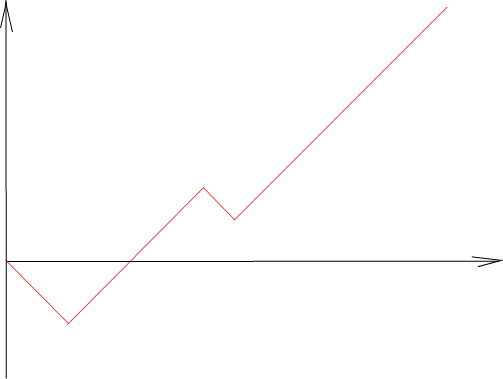
\includegraphics[width=.4\textwidth]{./pictures/4_4.png}
  \caption{График случайноо блуждания}
  \label{fig:44}
\end{figure}

$$S_n =
  \sum \limits_{i = 1}^n \varepsilon_i.$$
Найдём математическое ожидание этого процесса
$$MS_n =
  M \sum \limits_{i = 1}^n \varepsilon_i =$$
Пользуемся независимостью
$$= \sum \limits_{i = 1}^n M \varepsilon_i =
  0,$$
так как
$$M \varepsilon_i =
  1 \cdot \frac{1}{2} - 1 \cdot \frac{1}{2} =
  0.$$
Теперь найдём ковариационную функцию, то есть нужно найти
$$cov \left( S_m, S_t \right) =
  cov \left( \sum \limits_{i = 1}^n \varepsilon_i, \sum \limits_{j = 1}^t \varepsilon_j \right) =$$
Вынесем суммы за ковариацию
$$= \sum \limits_{i = 1}^n \sum \limits_{j = 1}^t cov \left( \varepsilon_i, \varepsilon_j \right) =
\sum \limits_{i, j = 1}^{n, t} M \left( \varepsilon_i \varepsilon_j \right) =$$
Такое математическое ожадине равно
$$M \left( \varepsilon_i \varepsilon_j \right) =
  \begin{cases}
    1, \qquad i = j, \\
    0, \qquad i \neq j.
  \end{cases}$$
Тут пар одинаковых чисел $ \min \left( n, t \right) $, так что
$$= \min \left( n, t \right).$$

По центральной предельной теореме
$$ \frac{S_n}{ \sqrt{n}} \to N \left( 0, 1 \right), \,
  n \to \infty,$$
потому что $S_n$ --- сумма независимых одинаково распределённых случайных величин.
